%
% Szakdolgozatminta az Eszterházy Károly Katolikus Egyetem
% matematika illetve informatika szakos hallgatóinak.
%

\documentclass[
% opciók nélkül: egyoldalas nyomtatás, elektronikus verzió
% twoside,     % kétoldalas nyomtatás
% tocnopagenum,% oldalszámozás a tartalomjegyzék után kezdődik
]{thesis-ekf}
\usepackage[T1]{fontenc}
\PassOptionsToPackage{defaults=hu-min}{magyar.ldf}
\usepackage[magyar]{babel}


%\usepackage{listingsutf8,mathtools,amssymb,amsthm,pdfpages,xurl}
\usepackage{listingsutf8,lmodern,caption,mathtools,amssymb,amsthm,pdfpages,xurl,float}


\footnotestyle{rule=fourth}

\newtheorem{tetel}{Tétel}[chapter]
\theoremstyle{definition}
\newtheorem{definicio}[tetel]{Definíció}
\theoremstyle{remark}
\newtheorem{megjegyzes}[tetel]{Megjegyzés}

\makeatletter
\expandafter\let\csname active@char\string?\endcsname\relax
\expandafter\let\csname active@char\string!\endcsname\relax
\expandafter\let\csname active@char\string:\endcsname\relax


\initiate@active@char{?}
\initiate@active@char{!}
\initiate@active@char{:}
\makeatother

\lstset{
    language=[Sharp]C,
    inputencoding=utf8/latin2,
    basicstyle=\footnotesize\ttfamily,
    columns=fullflexible,
    numbers=left,
    breaklines,
    xleftmargin=0.7cm,
    xrightmargin=0.7cm,
    frame=ltrb,
    rulecolor=\color{blue!80!black},
    backgroundcolor=\color{gray!30},
    commentstyle=\color{green!60!black},
    keywordstyle=\color{blue},
    morekeywords={using,public,class,int,void,new,for,bool,false,true,if},
}
\renewcommand{\lstlistingname}{kód}



\begin{document}

\institute{Matematikai és Informatikai Intézet}
\title{Mesterséges intelligencia elleni harci járműves játék készítése a NavMesh használatával}
\author{Pataki Tamás\\Programtervező Informatikus BSc}
\supervisor{Dr. Kovásznai Gergely\\Egyetemi docens}
\city{Eger}
\date{2025}
\maketitle

\tableofcontents

\chapter*{Bevezetés}
\addcontentsline{toc}{chapter}{Bevezetés}

A szakdolgozati témaválasztásom idején számtalan lehetőség közül válogathattam, de én olyan témát szerettem volna, ami egy sajátos kihívást ad és egyben az érdeklődési körömbe is tartozik. A számítógépes játékok és azoknak a fejlesztése már korábban is érdekelt, és ez adta meg az inspirációt egy új játék létrehozásához.

A témám egy olyan játék elkészítése, melyhez hasonlóval évekkel ezelőtt már játszottam, ebből hiányoltam néhány lehetőséget, és úgy gondoltam, hogy egy új tankos játék létrehozásában kifejezhetem saját kreativitásomat.

Emellett a harckocsik közötti csaták is érdekelnek, főleg a II. világháborúban használatos fegyverekkel. Emiatt egy olyan játékot szerettem volna fejleszteni, melyben megtapasztalhatjuk az akkori időben kifejlesztetett harckocsiknak az erejét. Csavarként gondoltam ki azt a funkciót, hogy a különböző harckocsik elemei megcserélhetőek legyenek egymás között, ezzel új lehetőségek nyílnak a taktikákra és ezzel további fantáziaelemeket próbálhatunk ki a játékban.

Emiatt választottam a projektem megvalósítására Unity\cite{unity} játékmotort, mely lehetőséget adott ennek kifejlesztésére 3D térben.

A szakdolgozatom az alábbi módon épül fel: az 1. fejezetben a tématerületet írom körbe és térek ki pár általánosabb fogalomra, amit használtam. A 2. fejezetben a konkrétabb felhasznált technológiákat és pár fontosabb funkciót mutatok be. Ezt követően a 3. fejezetben projek és annak működéséről lesz szó. Végül a 4. fejezetben a tesztelés menetét mutatom be.

A szakdolgozatom az alábbi linken érhető el: \url{https://github.com/patakitamas2002/Tank-Game}

\chapter{Tématerület áttekintése}

\section{Inspiráció}

Inspirációmat főként a War Thunder\cite{warthunder} című játékból merítettem, mely egy több mint 10 éve kiadott, de folyamatosan továbbfejlesztett, online többszereplős játék, melyben többféle járművet lehet benne irányítani - például repülőt, hajót, helikoptert, harckocsit. Az ötleteimet a harckocsis részéből merítettem. Több ezer jármú elérhető benne és mélyen kidolgozott rendszereik vannak, melyek a realizmusra törekednek. Ennek egy töredékét szerettem volna elérni egy félig realisztikus megoldással.


\begin{figure}[H]
    \centering
    \includegraphics[width=0.9\textwidth]{screenshots/warthundergame.png}
    \caption{Harckocsi modell Blender-ben}
    \label{fig:warthundergame}
\end{figure}


\section{NavMesh}

A NavMesh\cite{navmesh} a mesterséges intelligenciáknál alkalmazott absztrakt adatstruktúra, mely segít a komplex környezetekben történő útvonal keresésben. Ez a fogalom már több évtizede ismert a robotika területén, de a 2000-es évek elején népszerűsítették a számítógépes játékok.

Egy két-dimenziós konvex poligonokból\footnote{sokszögekből} álló háló adja meg az ügynök\footnote{Eredeti nevén \emph{agent}} által bejárható területet, melyen belül szabadon mozoghat. Egy poligonon belül egy egyenes vonallal lehet áthaladni, míg két poligon között gráfkereső algoritmusok használatával, mint például az A\* algoritmus, lehet útvonalat találni.

Egy NavMesh-t, bár lehet kézzel készíteni, nagyon hosszadalmas folyamat lenne, ezért általában egy pályán lévő statikus geometriában található magasság különbségek alapján van legenerálva.

A szakdolgozatom során tervezem ennek használatát a gépi ellenséges tankok irányításához.

\section{Ray cast}

A ray cast\cite{raycast}\footnote{Sugár követés} egy több évtizede kifejlesztett módszer a 3 dimenziós számítógépes grafikák megjelenítésére kétdimenziós képernyőkön. Ray cast segítségével el lehet dönteni, hogy adott nézőpontból melyik tárgy van előrébb.

Működése egy pontból kilőtt adott irányba haladó sugárral történik, mely visszaadja az első eltalált pontot, ezzel megállapítva, hogy az adott ponthoz képest mi található a legközelebb egy adott irányban.

Unity-ban ez egy beépített funkció és megadható a sugarak maximális távolsága, valamint az, hogy mely rétegeket vegye - vagy ne vegye - figyelembe.


\chapter{Felhasznált technológiák}

\section{Unity}

Fejlesztésem alapjául a Unity\cite{unity} játékmotort választottam népszerűsége és sokoldalúsága miatt. Rengeteg eszközt ad a fejlesztő kezébe, így szinte bármilyen típusú projekt elkészíthető vele, akár a játékfejlesztésen túl is.

\subsection{A Unity-ről általánosan}

A Unity először 2005-ben jelent meg, azóta a folyamatos továbbfejlesztés teljesen átváltoztatta. Jelenleg 2 és 3 dimenziós játékok fejlesztésére szolgál több platformon is, emellett interaktív szimulációkra használható és virtuális valóságra való fejlesztésre is van támogatása.

A fejlesztők részére bizonyos bevételig ingyenes lincensszel rendelkezik, emiatt az indie és újonc játékfejlesztők körében nagyon népszerűvé vált, tág közösségre tett szert, ezért többféle oktatóvideó található, és számtalan, a közösség által készített játékhoz tartozó elemet - pl. hangokat, modelleket - lehet letölteni vagy megvásárolni.

\subsection{Gameobject-ek}

Egyik alapeleme a Unity-nek a GameObject-ek\cite{GameObject}, melyeknek sokféle felhasználási módjuk van. A játékban bármelyik karakter, pálya vagy tárgy GameObject-nek számít egy jeleneten belül. Alapból nincsen konkrét funkciójuk, de komponenseket lehet hozzájuk csatolni, melyek meghatározzák a működésüket. Ezért a GameObjectet tekinthetjük úgy, mint egy tárolóegységet.

\subsection{Komponensek}

A komponensek\cite{components} felelnek a GameObject-ek viselkedéséért, rengeteg különféle funkcionalitást nyújtanak. Alapból több komponens van beépítve a Unity-be, de a szkriptelés kihasználásával saját komponenseket is lehet készíteni és ezzel a tár tovább bővíthető. A leggyakrabban használt beépített komponensek:
\begin{itemize}
 \item Transform\cite{transform} (Ezt minden GameObject tartalmazza)
 \item Mesh renderer\cite{meshrenderer}
 \item Collider\cite{collider}
 \item Rigidbody\cite{rigidbody}
 \item Szkriptek\cite{scripting}
\end{itemize}

A számtalan beépített komponens közül pedig az alábbiakban emelném ki a legalapvetőbbeket:
A \emph{Transform} adja meg a pozícióját, méretezését és forgatását az adott objektumnak, a modellek megjelenítésért a \emph{Mesh renderer} felel. A \emph{Collider} az ütközések kezelését szolgálja, több formában is létezik, mint például doboz és kapszula alakú. A \emph{RigidBody} felel a fizikáért.

\subsection{Szkriptelés}

A szkriptek egyféle komponensei a GameObjectnek. A játék logikájának és interakcióinak megírására szolgálnak. A szkriptek főként C\# nyelven készülnek, és az egyes játékobjektumok viselkedését, mozgását valamint a játékbeli eseményeket szabályozzák.


A \emph{MonoBehaviour} nevű osztályból öröklődik a legtöbb szkript, mely többféle beépített életciklust tesz elérhetővé:

\begin{itemize}
    \item \emph{Start}
    \item \emph{Update}
    \item \emph{FixedUpdate}
    \item \emph{OnCollisionEnter} / \emph{OnTriggerEnter}
\end{itemize}

Az adott objektum betöltődésénél a \emph{Start} metódus a szkript indításakor egyszer fut le, amennyiben a szkript engedélyezve van. A \emph{Start} metódust általában inicializálási feladatokhoz alkalmazzák, például változók értékeinek beállítását hajtja végre.

Az \emph{Update} metódus minden képkockánál lefut, így ide kerülnek azok a kódok, amelyeknek folyamatosan, valós időben kell futniuk, például a mesterséges intelligenciák irányítása vagy a kezelőfelületen lévő folyamatosan frissülő részek.

A \emph{FixedUpdate}, az \emph{Update}-hez hasonlóan, folyamatosan fut, viszont minden fizikai képkockán fut le, a megjelenített képkockáktól függetlenül. Ide a fizikai számítások kerülnek, mivel megadott időközönként fut újra.

Az \emph{OnCollisionEnter} akkor fut le, amikor két \emph{Collider} komponenssel rendelkező tárgy összeütközik. A \emph{OnCollisionEnter} az ütközések vagy fizikai lövedékek kezelésére alkalmas.


\section{Blender}

A modellezéshez Blender-t választottam, mely egy ingyenes és nyílt forráskódú 3D modellező és animációs program. A Blender egy nagyon széles körben használt és alkalmazott program a 3D grafika világában, és ingyenessége miatt bárki számára   hozzáférhető és kipróbálható.

\begin{figure}[H]
    \centering
    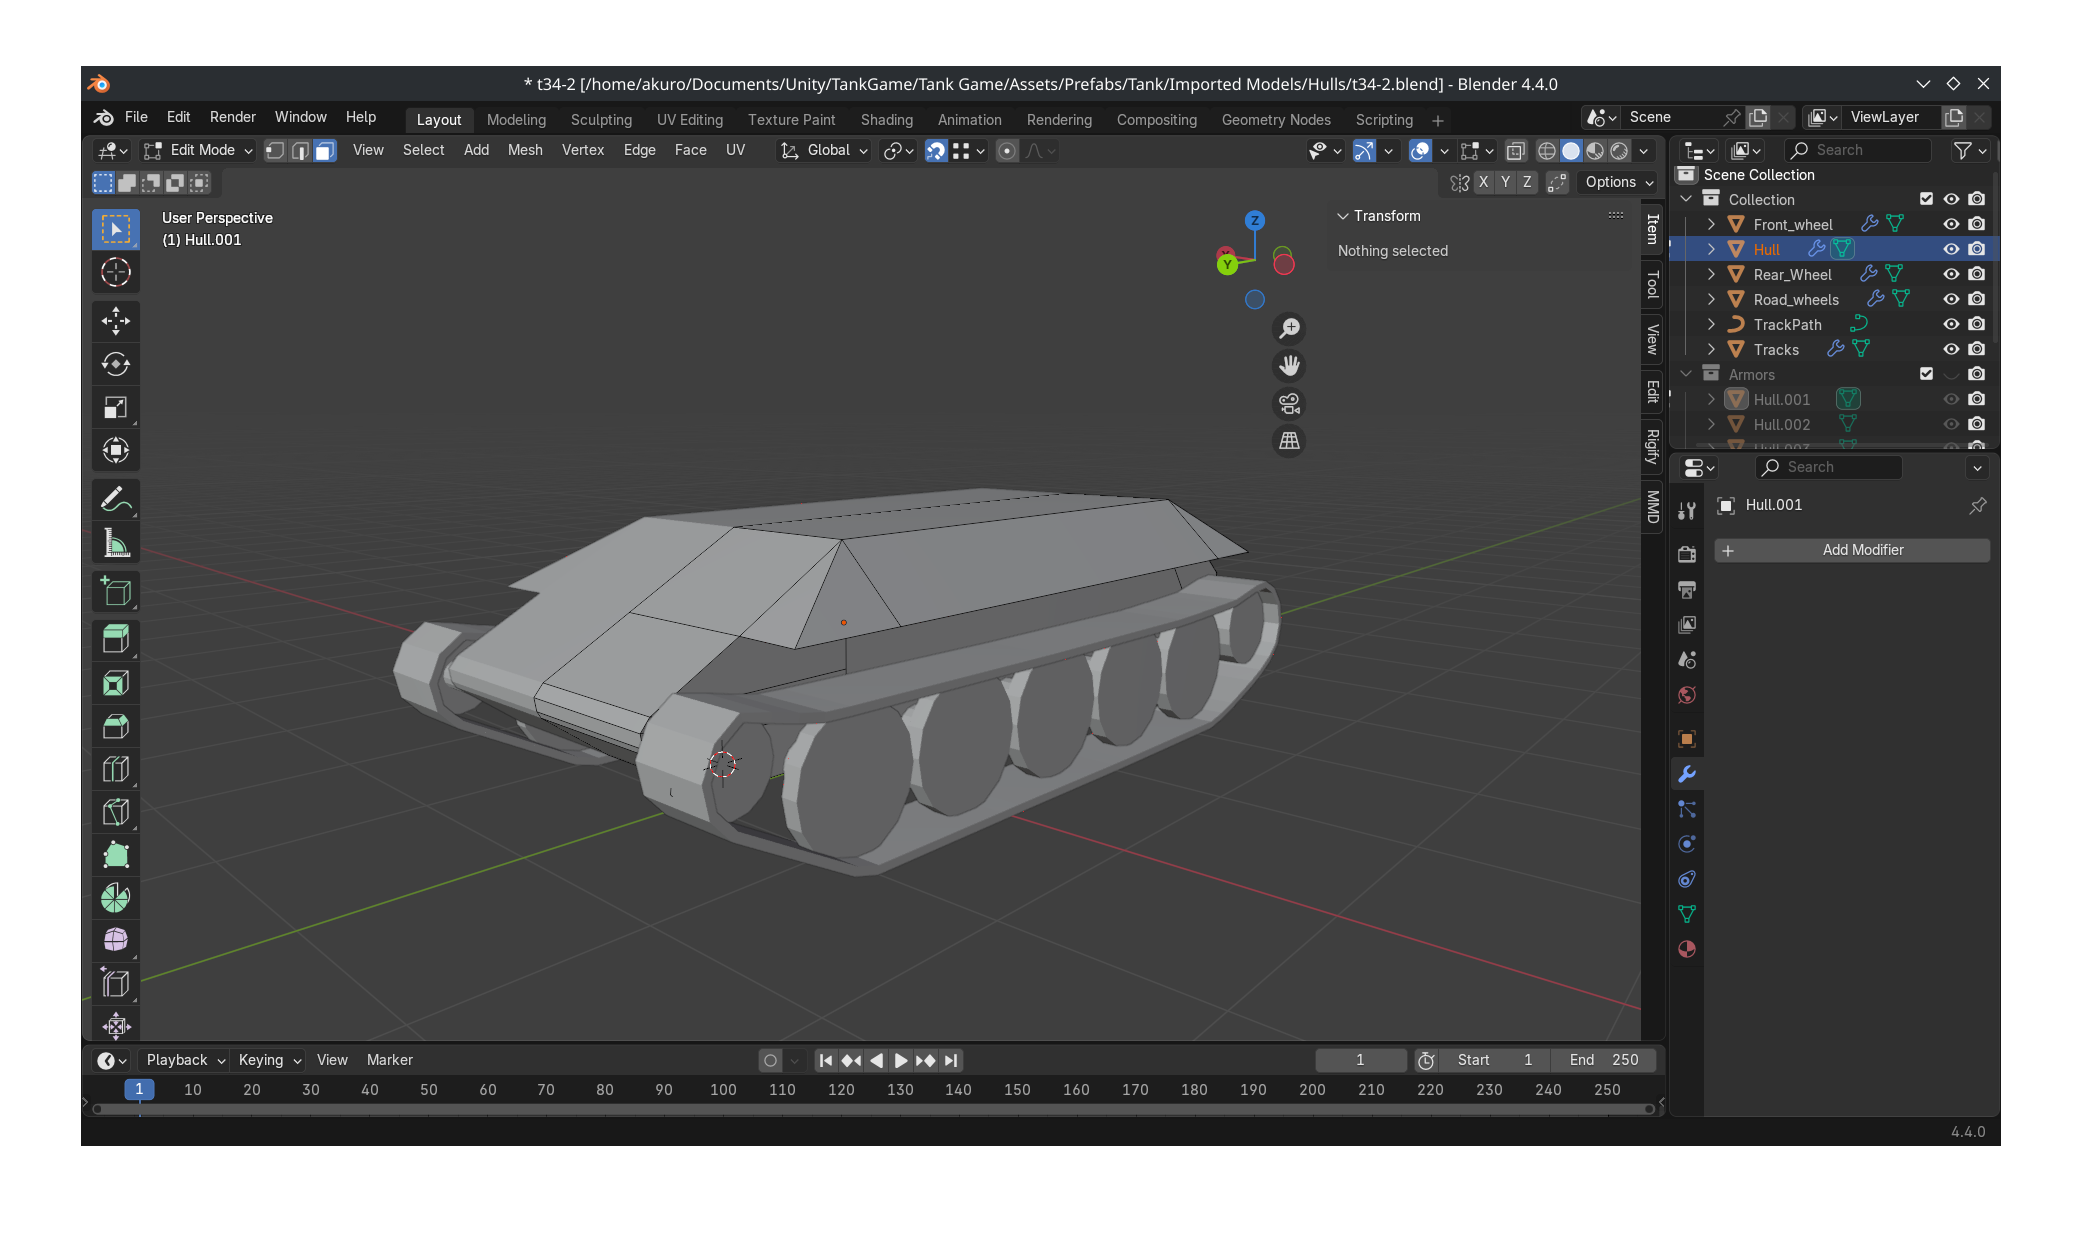
\includegraphics[width=0.9\textwidth]{screenshots/blender.png}
    \caption{Harckocsi modell Blender-ben}
    \label{fig:blender}
\end{figure}

A Blender újabb verzióiban számtalan eszköz elérhető, ami egyszerűbbé teszi a modellezést és annak tanulását, mindemellett a felhasználói közössége miatt több segítség is található internetes fórumokon, valamint sok tanító videó is rendelkezésre áll. Mindez nagy segítséget nyújtott számomra a program használatában.

\chapter{A játék bemutatása}

\section{A játékmenet}

\subsection{Menü}

A játék betöltődését követően a főmenübe kerülünk, ahol 3 gomb található:
\begin{itemize}
 \item Play (tank kiválasztása)
 \item Settings (beállítások)
 \item Exit (kilépés)
\end{itemize}

A Play gombra kattintva megjelenik a harckocsi kiválasztására szolgáló menü, és itt a felső részen a gombok segítségével kiválaszthatjuk a harckocsi részeit, melyek megnevezése a gombok között található. A képernyő közepén láthatjuk a jelenleg kiválasztott harckocsi előnézetét, amely az alkatrészek cseréje során frissül, így a létrehozott tankot azonnal láthatjuk.

A játék indító gombja (\emph{Start mission}) a képernyő jobb alsó sarkában található, míg a bal alsó sarokban a főmenübe visszalépő gomb (\emph{Back}) van.


\begin{figure}[H]
    \centering
    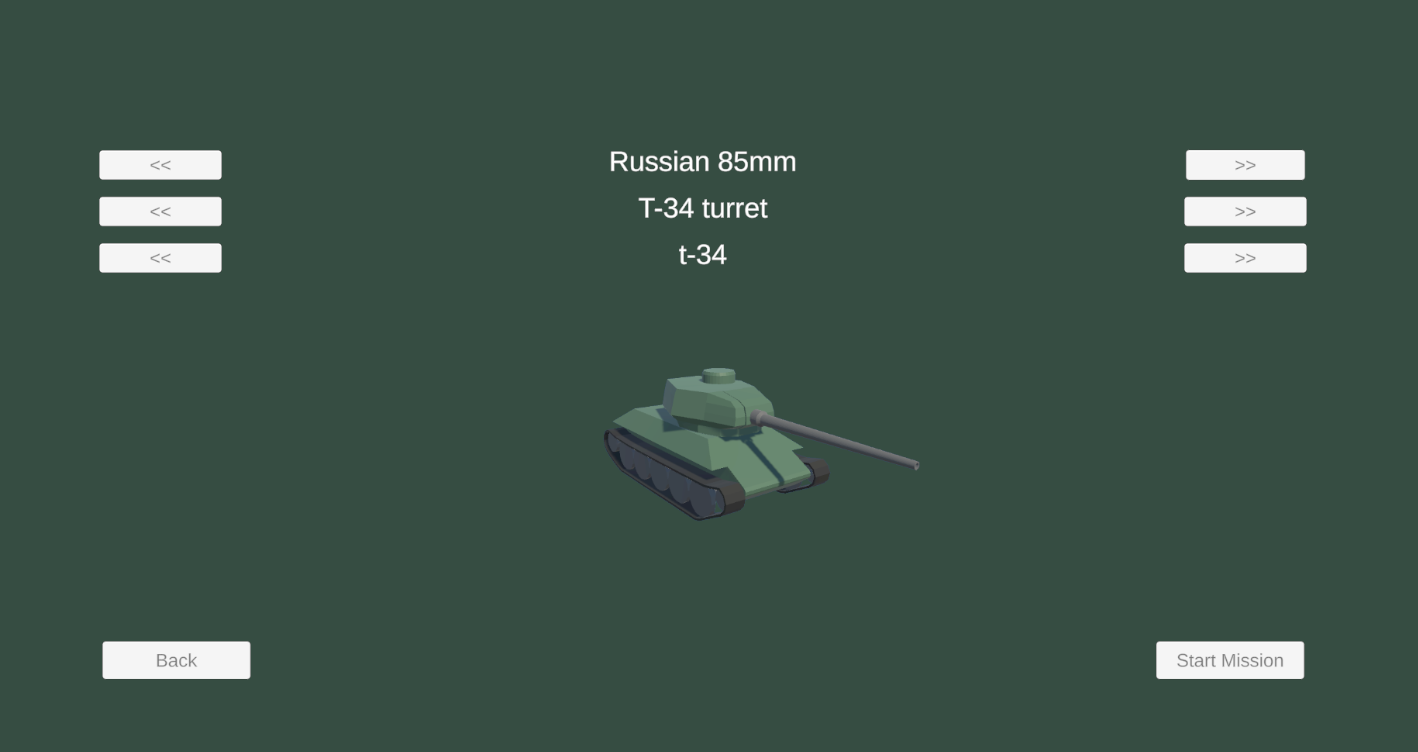
\includegraphics[width=0.7\textwidth]{screenshots/selectionmenu.png}
    \caption{Harckocsi választási menü}
    \label{fig:selectionmenu}
\end{figure}

A beállításoknál 3 csúszka található, melyek mellett a jelenlegi értékük jelenik meg. Ezek a csúszkák szolgálnak a játékbeli érzékenység és a hangerő beállítására.

\begin{figure}[H]
    \centering
    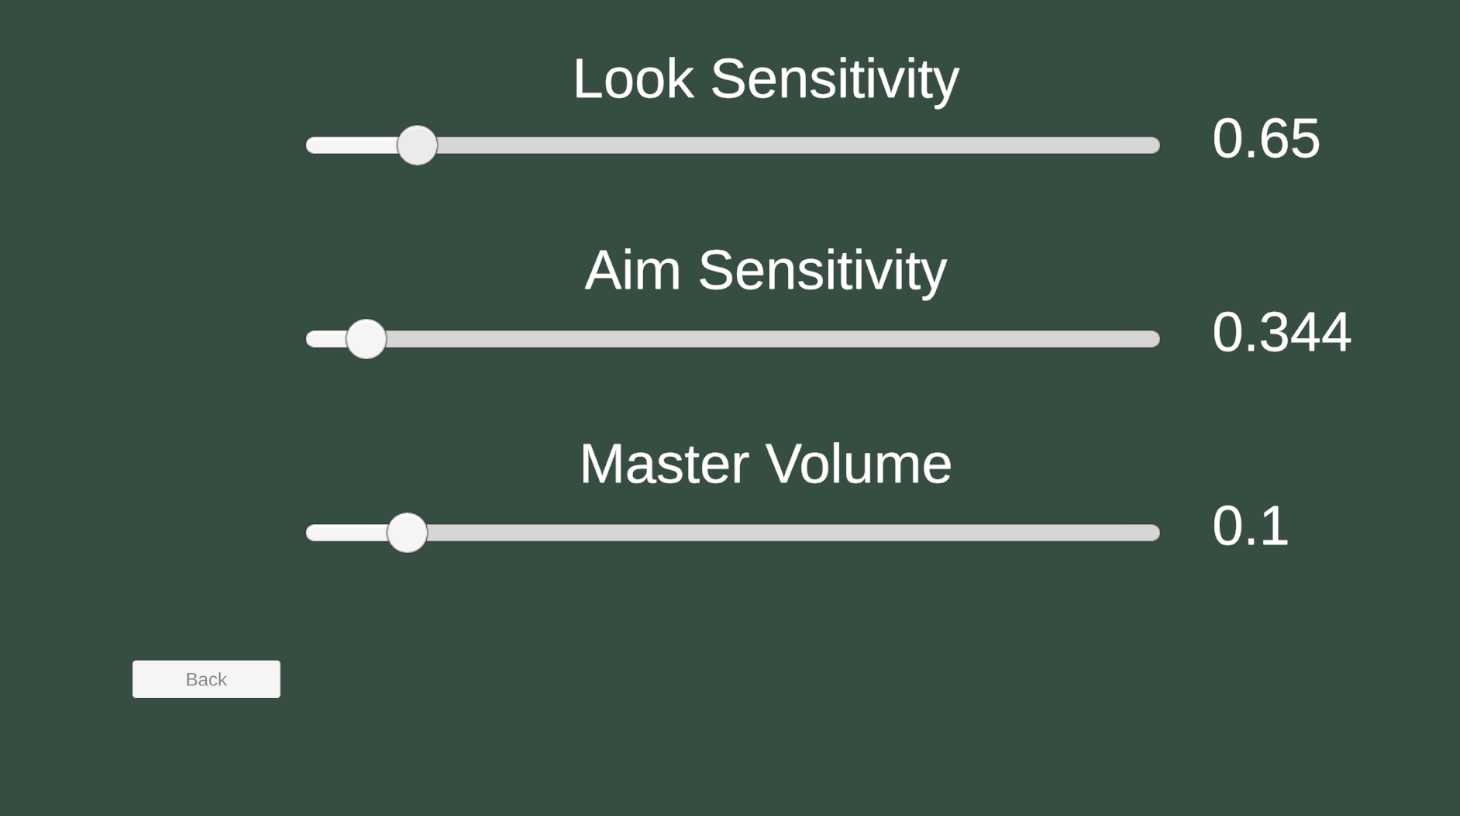
\includegraphics[width=0.7\textwidth]{screenshots/settings.png}
    \caption{Beállítási menü}
    \label{fig:settings}
\end{figure}

\subsection{Csata}

A harckocsi kiválasztását követően elindul a csata, ahol egy sziklás pályán jelenik meg a játékos tankja, és az ellenséges harckocsik egy útvonalat követve indulnak meg a  célpontjukig. A játékos célja, hogy az ellenfeleket megsemmisítse, mielőtt a célpontjukhoz érnének. Ha bármelyik ellenfél eléri a célpontot vagy a játékos harckocsija megsemmisül, akkor a játékos veszít.

\section{A megvalósítás}

\subsection{A harckocsi}

A \emph{Tank} komponens sok dologért felel, leginkább a különböző részek létrehozásáért, statisztikáiknak az összekombinálásáért és az életerő-t is kezeli.

\lstinputlisting[caption=A harckocsi létrehozása,label=tankspawn]{./codesnippets/tankspawn.cs}

A \emph{CreateTank} metódus először a gyökér objektumot hozza létre, melyhez hozzáadja a \emph{Tank, Rigidbody} és \emph{BoxCollider} komponenseket. Ezt követően a harckocsi alkatrészeit létrehozza gyerek objektumokként, melyek a többi alkatrész által megadott pozíciókba kerülnek.

Ez a komponens egyéni tapadási fizikáért is felel, mely nagyobb sebességgel történő fordulásnál jelentősen lecsökkenti a harckocsi sebességét, így az kívánt irányba halad tovább. Ennek hiányában forduláskor nem lenne tapadás és a tank oldalirányban csúszna. A \emph{SidewaysFriction} a \emph{FixedUpdate}-ben csak akkor fut le, ha a harckocsinak legalább az egyik lánctalpa a földön van.

\lstinputlisting[caption=Tapadási kód,label=tracion]{./codesnippets/traction.cs}

A kód az oldalirányú mozgási sebességtől függően - melyet a mozgási irány vektor és az oldal irányú vektor szorzatából kap meg - csökkenti a sebességet a \emph{sidewaysFrictionFactor} alapján. Az értéket tesztelés és érzés alapján állítottam be.

A harckocsi 3 részre van felosztva:
\begin{itemize}
    \item Páncéltest
    \item Lövegtorony
    \item Ágyú
\end{itemize}

Ezen túlmenően ha a harckocsi élete 0 vagy annál kisebb értékre csökken le, akkor megsemmisültnek számít, melyet abból vehetünk könnyen észre, hogy ebben az esetben a lövegtorony lerepül a páncéltestről.


\subsubsection{Páncélzati rendszer}
Minden harckocsi modellje fel van osztva több kis darabra, melynek van a beépített \emph{Collider} komponense és a saját páncél komponense. Ezzel a módszerrel pontosan meg lehet adni, hogy melyik részen mekkora védelme legyen és mekkora sebzési szorzót kapjon. Például az ágyúnak és a lánctalpnak kisebb a szorzója, mivel könnyebben átüthető részeknek számítanak, így a harckocsi középpontja ebben az esetben nem sérül. Az ötletet az alábbi projekt\cite{armoridea} alapján kaptam.

\subsubsection{Páncéltest}

Általánosságban ez rendelkezik a legtöbb páncél elemmel, valamint a páncéltest adja meg a tankon a lövegtorony elhelyezkedését, továbbá ez adja meg az egész harckocsi maximális sebességét, gyorsulását, a motor hangját és az életerejének a nagy részét. Ezen túlmenően ehhez tartoznak a lánctalpak is, melyek ellenőrzik, hogy a harckocsi a földön van-e az adott pillanatban, amit  egy rövid \emph{ray cast} segítségével érzékel.

\subsubsection{Lövegtorony}

A lövegtorony forgatását a játékos nézőpontjából kilőtt sugár segítségével implementáltam, mely visszaad egy koordinátát, és miután a lövegtorony ezt megkapja, elkezd fordulni megadott sebességgel a kívánt irányba. Emellett a lövegtorony adja meg a belső kamera pozícióját és az ágyú elhelyezkedését is.

\lstinputlisting[caption=Lövegtorony forgatása,label=turretrotation]{./codesnippets/turretrotation.cs}

A \emph{RotateTowards} metódus először megkap egy vektort a célpont pozíciója és a torony pozíciójából, amiből kiszámítja a kiválasztott irányt. Ezután megkapja \emph{Quaternion}-ban a forgási irányt és végül elkezdi forgatni a tornyot másodpercenként \break
\emph{stats.RotationSpeed} által megadott fokkal. Alapul az alábbi kódrészletet\cite{rotation} vettem.

\subsubsection{Ágyú}

Az ágyú emelése is hasonlóan működik a torony forgatásához képest, viszont megadott a maximum magassági és depressziószöge, melyeket nem léphet túl a függőleges fordulása. Valamint az ágyú adja megy, hogy a játékos számára milyen lőszerek elérhetőek.

\lstinputlisting[caption=Lövegtorony irányítása,label=barrelelevation]{./codesnippets/barrelelevation.cs}

A kódban sincs túl nagy eltérés a torony forgatásához képest. Viszont itt a 2. sorban a Pitagorasz-tétel\cite{pitagorasz} alkalmazásával a távolságot kiszámítja, utána annak segítségével kapja meg a kívánt szöget, és itt figyelembe veszi azt is, ha a harckocsi emelkedőn van-e. A forgatási limit a 7. sorban van megadva.


\subsubsection{Játékos nézőpontja}

A játékos nézőpontját 2 darab kamerával oldottam meg, külső és belső nézetessel, melyeknek az érzékenységét külön-külön lehet beállítani. Az egérgörgővel lehet csökkenteni a kamera látószögét, mely segíthet a nagyobb távolságra történő célzásban.

\subsection{Pálya}

\subsubsection{Kialakítása}

A pálya kialakításához a Unity terepszerkesztőjét használtam, mely az ecsetszerű eszközök segítségével a terepen magasabb és mélyebb részek rajzolására volt lehetőség, és ennek használatával egy hegyes-dombos pályát készítettem egy kivájt útvonallal.
\subsubsection{Textúrázás}

A textúrázást szintén a terepszerkesztő eszközzel készítettem, mellyel az útvonalat egy ecsettel van lehetőségünk festeni. A textúrákat a \emph{Poly Haven}\cite{polyhaven} oldalról töltöttem le.

\begin{figure}[H]
    \centering
    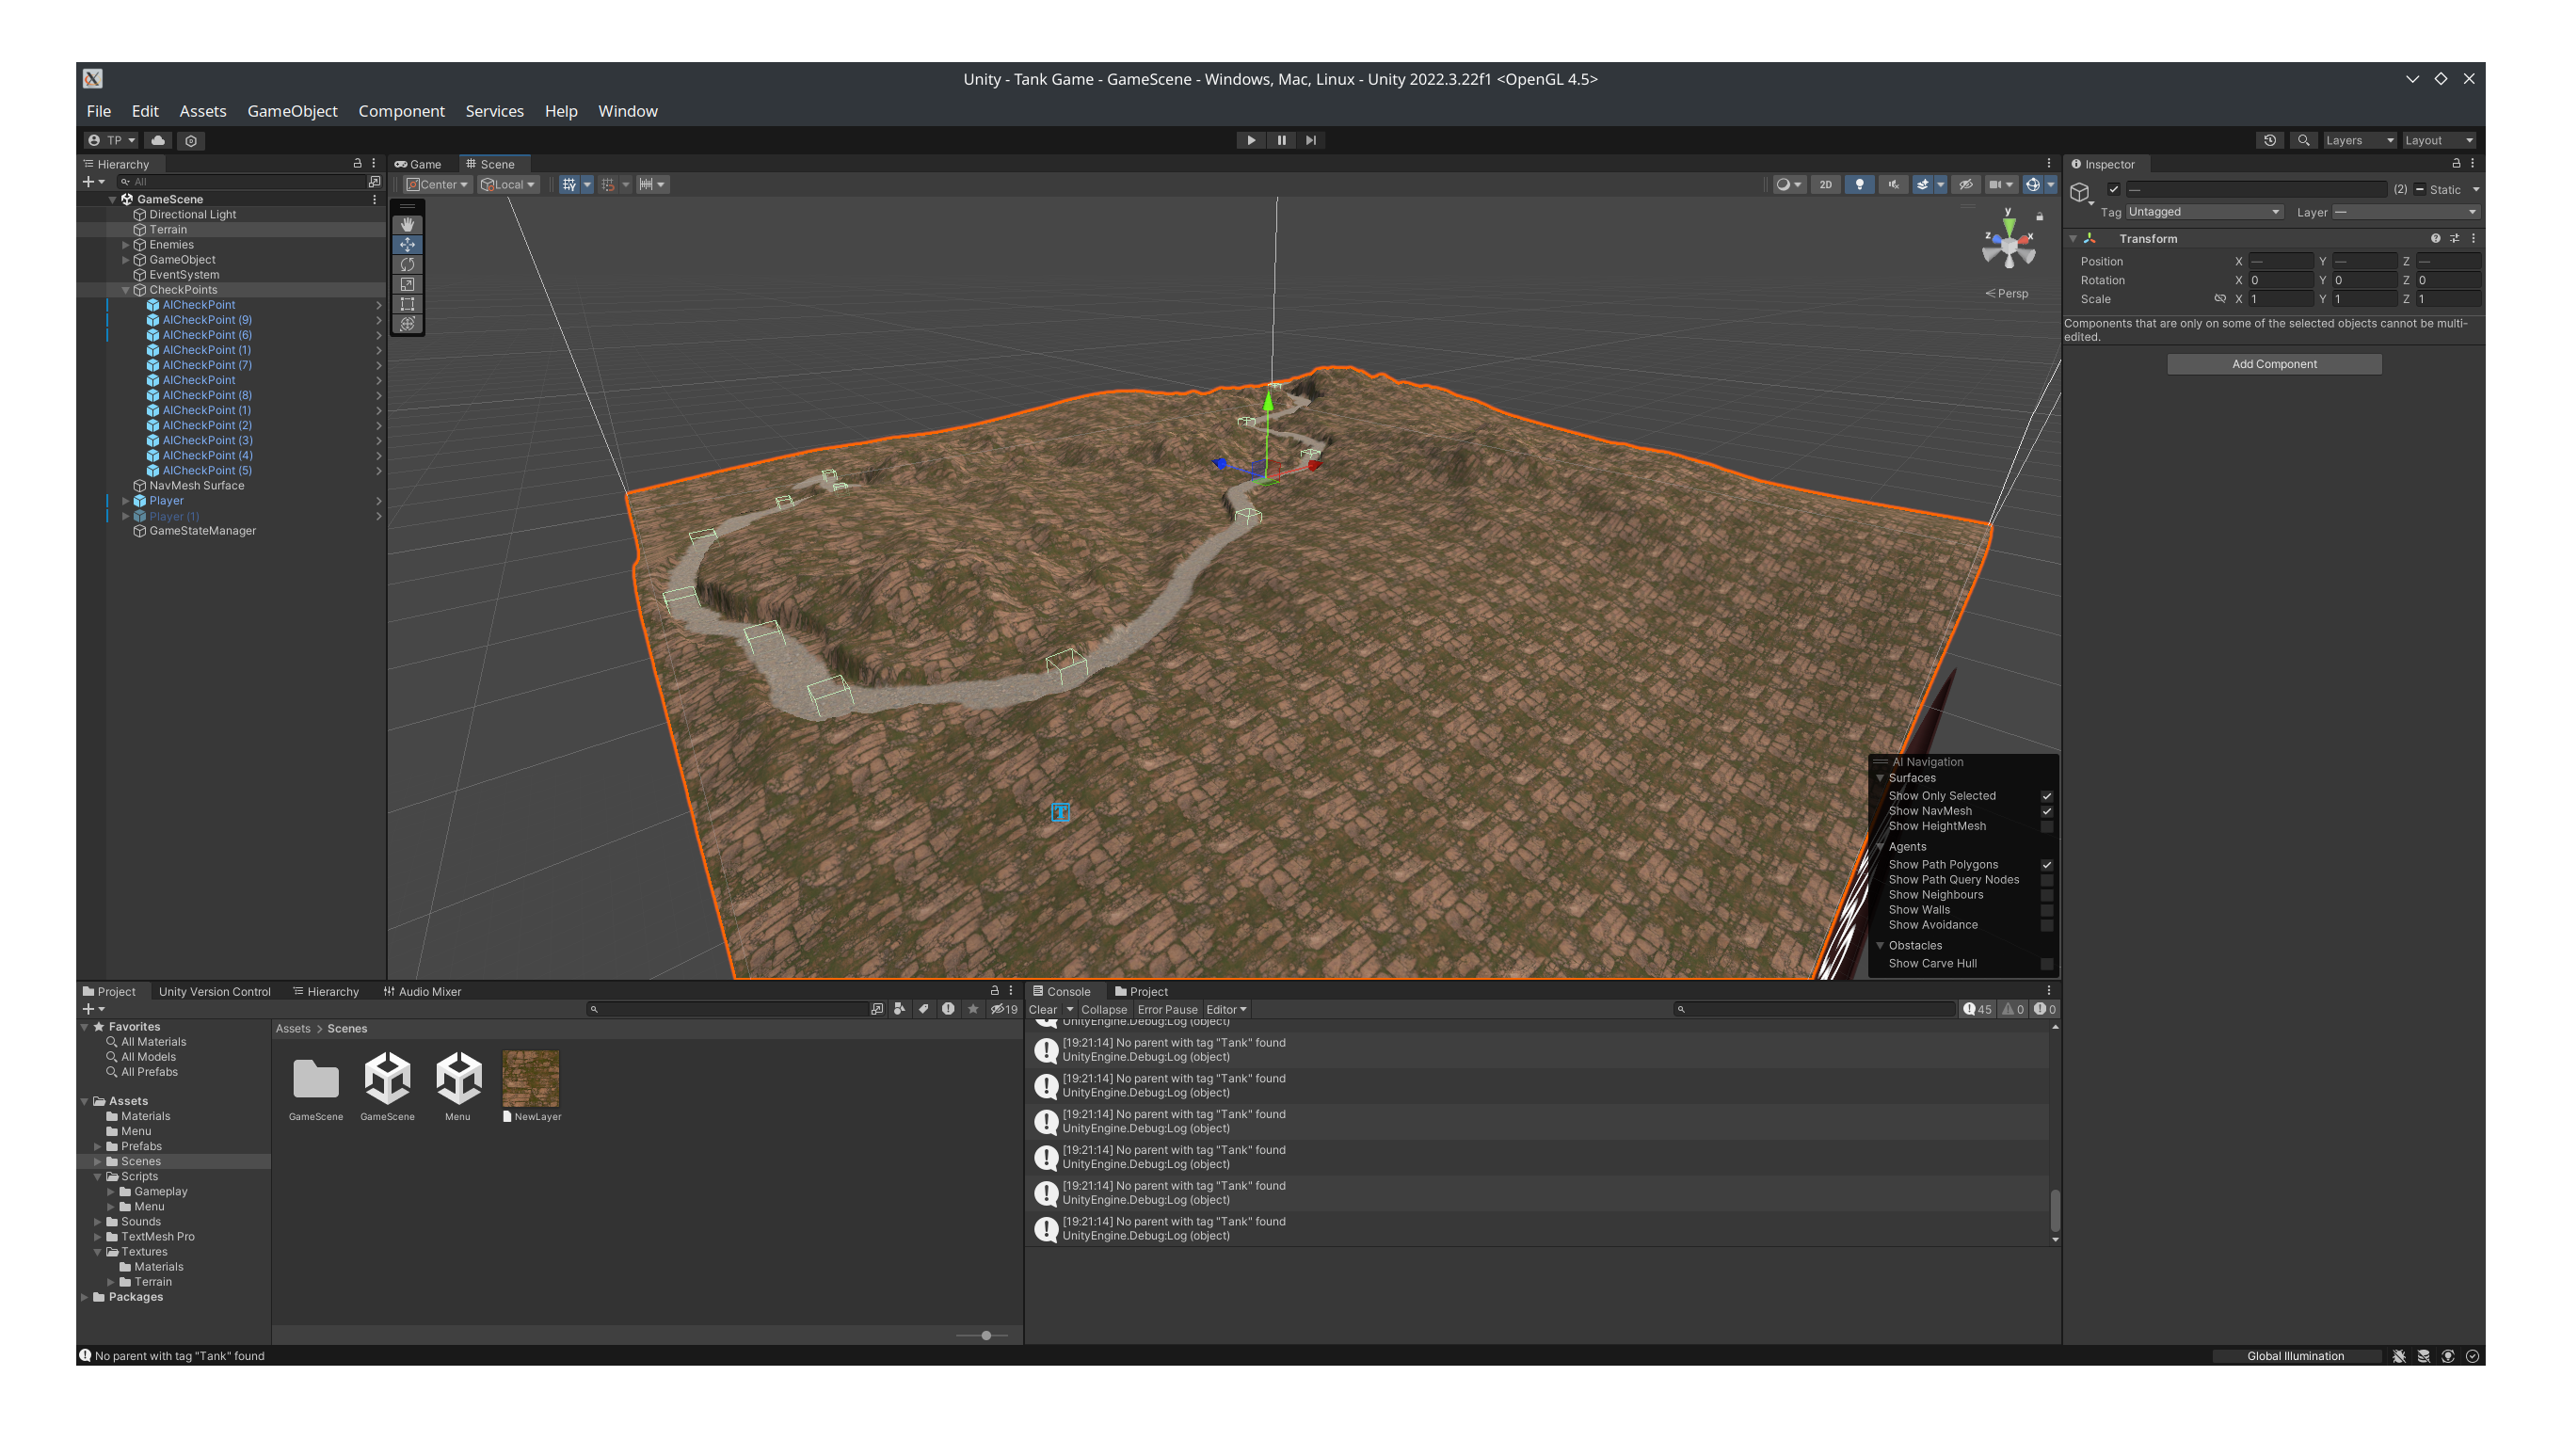
\includegraphics[width=0.8\textwidth]{screenshots/mapineditor.png}
    \caption{A Unity szerkesztőjében a pálya}
    \label{fig:mapineditor}
\end{figure}

\subsection{Menü}

\subsubsection{Harckocsi kiválasztása}

A harckocsi részeit a Unity-ba beépített \emph{ScriptableObject}-ek segítségével tudjuk eltárolni, majd a későbbiekben a játék során elérni. A kiválasztási rendszerhez az ötletet az alábbi videó\cite{selectionmenu} adta.

\begin{figure}[H]
    \centering
    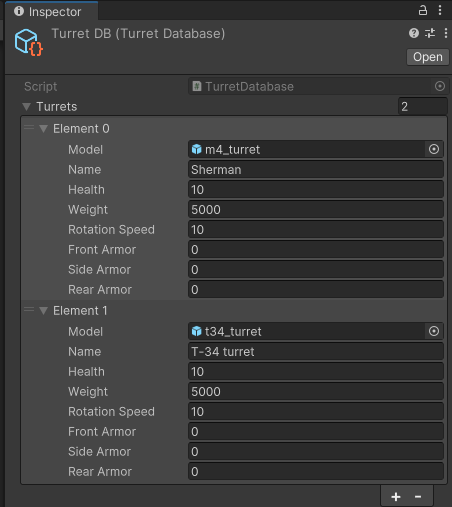
\includegraphics[width=0.5\textwidth]{screenshots/scriptableobject.png}
    \caption{\emph{ScriptableObject} kezelőfelülete}
    \label{fig:scriptableobject}
\end{figure}


\subsubsection{Beállítások}

A beállítások menüben az érzékenység és a hangerő beállítására van lehetőségünk a csúszkák mozgatásával, amelyek értékei egy statikus osztályban tárolódnak el.


\subsubsection{Szünet menü}

A játékban létrehoztam egy ún. szünet menüt - ebben az esetben a játékmenet leáll - viszont bármikor folytatni tudjuk, de lehetőségünk van elölről kezdeni a csatát, vagy visszalépni a főmenübe.

\subsection{Irányítási rendszer}

A bevitelhez a Unity új beviteli rendszerét használtam segítségül, melynek használatával egyszerűen lehetett újabb beviteli billentyűket hozzáadni, valamint azokat csoportosítani és együttesen ki- vagy bekapcsolni. Az alábbi videó\cite{inputsystem} alapján készítettem el ezt a rendszert.

\subsubsection{Célzás}

Az egér mozgatásával tudunk célozni, és bár a játékmenet közben a kurzor nem látható, mivel ez a játékablak közepére van lerögzítve, de mindaddig úgy marad, amíg a játékos meg nem nyitja a szünet menüt vagy véget nem ér a játékmenet.

\subsection{Lövedékek}

A lövedékek fizikai objektumként működnek, megadott sebességük és súlyuk van, de a gravitáció nincs hatással rájuk.

A játékban jelenleg háromféle lövedék elérhető:
\begin{itemize}
    \item páncéltörő
    \item robbanótöltetes pácéltörő
    \item robbanótöltetes lövedék
\end{itemize}

Mindhárom típus egy absztrakt \emph{Bullet} osztályból öröklődik, így a \emph{Start} és az \emph{OnCollisionEnter} metódusaik közösek, valamint implementálniuk kell a \emph{GetMaxPenetration, CalculateDMG} és \emph{CalculatePenetration}-t.

\lstinputlisting[caption=Absztrakt \emph{Bullet} osztály metódusai,label=bullet]{./codesnippets/bullet.cs}

A \emph{Start} metódusban beállítja a kezdeti pozíciót, az átütési értéket, a sebességet és a méretét a lövedéknek. Az alaplövedék modellje 100mm átmérőjű, és emiatt a lövedék pontos méretét úgy kapja meg, hogy az adott lövedék méretét kaliberével beszorozza, és azt elosztja százzal.

Az \emph{OnCollisionEnter} ütközéskor fut le, ellenőrzi hogy ütközött-e páncéllal. \break
Amennyiben igen, akkor nem történik további sebzés. Más esetben megvizsgálja, hogy az ütközés páncéllal történt-e, és kiszámítja a kezdeti pozíciótól megtett távolságot. Amennyiben páncélnak minősül az eltalált objektum, kiszámításra kerül a megmaradt átütőerő, és ha még mindig maradt átütési erő - azaz a páncél nem állította meg a lövedéket -, az ellenfél sebzést szenved el.


\subsubsection{Páncéltörő lövedék}

A páncéltörő lövedéket a DeMarre-formula alapján modelleztem. A képlet a tömeg, az átmérő és a sebesség alapján számítja ki a lövedék maximális átütési erejét.

%DeMarr Formula
\begin{equation}
 P_r \times \left( \frac{V}{V_r}\right)^{1,4283} \times \left( \frac{D}{D_r} \right)^{1,0714}  \times \left(\frac{W}{\varnothing}\right)^{0,7143} \div \left(\frac{W_r}{\varnothing_r}\right)^{0,7143}
 \label{demarre}
\end{equation}


A lövedéknek figyelembe vesszük a megtett távolságát és a találati szögét is. Ezen a tényezők hatását kettő változóval lehet befolyásolni, \emph{DistanceFalloff}-fal és \emph{AnglePerformance}-szel. Amennyiben a \emph{DistanceFalloff} értéke 1 a távolság nem befolyásolja az átütőképességet. 1 alatti értéknél, melyet a legtöbb lövedék használ, a távolság függvényében csökken az átütőerő, míg az 1 feletti értéknél nő. Az \emph{AnglePerformance}-nál a 0-ás érték figyelmen kívül hagyja a találati szöget. Ezzel szemben az 1-es értéknél a páncélvastagság találati szögből adódó növekedését $\cos$ függvény alapján számítja ki. A leggyakrabban használt 1 feletti érték gyengíti az átütőerőt nagyobb szög esetén. Amennyiben a \emph{DistanceFalloff} és \emph{AnglePerformance} értékeket 1-re állítjuk, abban az esetben egy eltérő viselkedésű lövedéktípust kapunk.


\lstinputlisting[caption=Átütés kiszámítása,label=APcalculation]{./codesnippets/APcalculation.cs}

A lövedék sebzését - melynek maximális értéke kaliberétől és a sebességétől függ - az átütött páncél értékéhez és a lövedék átütő erejétől függően csökkentjük.

\subsubsection{Robbanótöltetes lövedék}

Az alábbi lövedék egy felülethez érve egy robbanást szimulál, melynek során megadott távolságon belül először megvizsgálja az összes objektumot, azt, hogy melyik számít páncélnak. Ezt követően kiszámítja,hogy a páncéllemezek közül melyik a leggyengébb, a lemez vastagsága és a a robbanás középpontjából számított távolságának kombinációjából.

\lstinputlisting[caption=Robbanótöltetes lövedék működése,label=hexplosion]{./codesnippets/heexplosion.cs}

A \emph{GetMaxPenetration} függvény egy egyedi módszert alkalmaz az átütés kiszámítására. Az értékeket a \emph{War Thunder} lövedékéihez hasonlóan szerettem volna megvalósítani, de végeredményben a számításom eltérő értékeket ad.

A \emph{CalculatePenetration} függvény a leggyengébb páncél alapján adja vissza a maradandó átütést. Ehhez a \emph{GetWeakestArmor} metódust alkalmazza, mely először megvizsgálja az összes \emph{Collider}-el rendelkező objektumot egy adott távolságon belül. Ezután \emph{Ray cast}-ok használatával vizsgálja meg. hogy a robbanás középpontjából látható-e az adott objektum, melyet a pozícióik összehasonlításával ellenőriz - figyelmen kívül hagyva a \emph{CollisionBox} réteget. Amennyiben az adott objektum páncél, akkor kiszámítja az ellenállását a \emph{GetResistance} függvénnyel, mely a távolság függvényében növeli a páncél védelmének erejét négyzetesen.


\subsubsection{Robbanótöltetes páncéltörő lövedék}

Ez a lövedék a sima páncéltörő lövedékhez képest hasonlóan működik, mivel az átütő ereje szintén a \emph{DeMarre} formula alapján került kiszámításra. A különbség a sebzés módszerében rejlik, ami csak akkor eltérő, ha a lövedék megadott érzékenységénél vastagabb páncélt ütött át, és ezt követően a robbanótöltet mértékétől függően sebez.


\subsection{Kezelőfelület}

\subsubsection{Életerő sáv}

A projektben kétféle életerő-sávot készítettem: Az első típus a kezelőfelületen található a bal alsó sarokban, ahol számokkal jelzi ki a teljes és a jelenlegi életerőt. A második típus az ellenségek felett található meg, mely 3D térben helyezkedik el, követve az egység pozícióját. Az alsó és felső sáv is a mutatja külön-külön az adott egység megmaradó életerejét.
\begin{figure}[H]
    \centering
    
\includegraphics[width=0.5\textwidth]{screenshots/hpbar.png}
    \caption{Életerő sávok}
    \label{fig:healthbar}not
\end{figure}


\subsubsection{Célkereszt}

A célkereszt 2 részből áll. A kör alakú irányzék a képernyő közepét és a kívánt célpontot jelöli, amely lövés után pirossá változik, utána folyamatosan kezd kitöltődni fehér színnel, jelezve az újratöltés folyamatát. A második ``kereszt'' alakú, pedig azt jelzi, hogy a cső pillanatnyilag melyik irányba néz.

\begin{figure}[H]
    \centering
    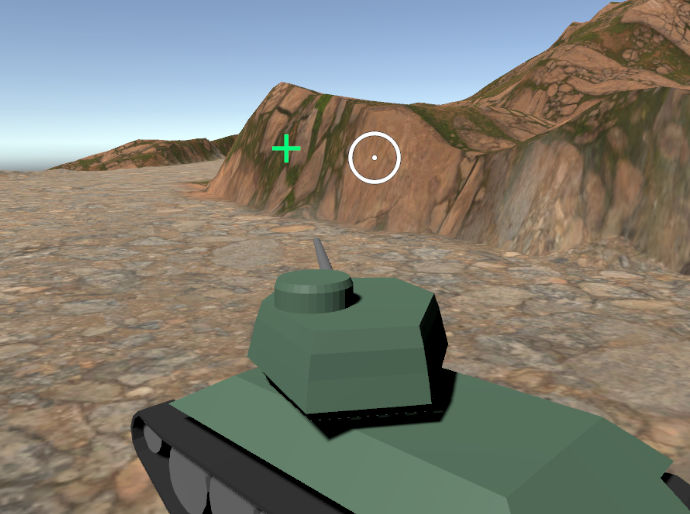
\includegraphics[width=0.5\textwidth]{screenshots/crosshair.png}
    \caption{Célkeresztek}
    \label{fig:crosshair}
\end{figure}

\subsection{Hangok}

A játékban jelenleg kétféle hang hallható: a motor- és a lövéshang. A motorhang folyamatosan ismétlődik, hangmagassága a jármű sebessége alapján növekszik vagy csökken. A lövéshang csak lövés esetén hallható. A hangokat az alábbi oldalról\cite{freesound} töltöttem le.

\subsection{Ellenfelek}

\subsubsection{NavMesh}

Az ellenségek útkeresését a Unity beépített NavMesh rendszere segítségével valósítottam meg. A Unity NavMesh lehetőséget biztosít az egység irányítására is, azonban alapvatően emberszerű karakterekre mozgatására lett tervezve. Emiatt a harckocsik mozgatásához egy egyedi megoldást kellett implementálnom, amely eredményeként az ellenfelek ugyanazt a mozgásrendszert használják, mint a játékosok.

\subsubsection{Ellenőrzőpontok}

Az ellenségek egy előre meghatározott útvonalat követnek, amelyet a játékos számára láthatatlan ellenőrzőpontok segítségével valósítottam meg. Amikor az ellenség belép egy ellenőrzőpontba, az alábbi kódrészlet fut le, amely először ellenőrzi, hogy az ellenség az aktuális célpontján haladt-e át. Amennyiben igen, a rendszer beállítja következő célpontot.

\lstinputlisting[caption=Ellenőrző pontok váltása,label=checkpoints]{./codesnippets/checkpointsystem.cs}


\subsubsection{Állapotgép}

Az ellenfelek viselkedését ún. állapotgép segítségével szabályoztam, amelyet a tiszta felépítése és egyszerű bővíthetősége miatt választottam.

\lstinputlisting[caption=Lövegtorony irányítása,label=statemachine]{./codesnippets/statemachine.cs}

\subsubsection{Állapotok}

Kétféle állapot van:
\begin{itemize}
 \item Járőrözés
 \item Támadás
\end{itemize}

\subsubsection{Járőrözés}

Az alapértelmezett állapot a járőrözés, ebben az esetben az ellenség az ellenőrző pontok által meghatározott útvonalat követi. A két ellenőrző pont közötti útvonalat a NavMesh segítségével kerül meghatározásra.

\subsubsection{Támadás}

Az ellenség akkor vált a támadási állapotba, ha a játékos egy adott távolságon belül elhalad előtte. Amíg a játékos nem kerül akadály mögé, az ellenség a páncéltestét és a tornyát a játékos irányába forgatja. Miután a játékost sikeresen célba vette, az ellenség lő. Ha a játékos kimegy az ellenség maximális észlelési távolságából vagy egy akadály mögé bújik, az ellenség megpróbálja utolérni a játékost. Ilyenkor egy időzítő is elindul, és ha egy meghatározott időn belül a játékos nem kerül elő, akkor az ellenség visszatér a járőrözési állapotba.

\lstinputlisting[caption=Állapotgép,label=checkplayervisible]{./codesnippets/checkplayervisible.cs}

A játékos láthatóságának vizsgálatát a \emph{CheckPlayerVisible} függvény végzi, amely először a játékostól való távolságot ellenőrzi. Ha ez a távolság a megadott küszöbérték alá esik, akkor egy vektor segítségével kiszámítja a játékos felé mutató irány szögét. Ezt követően megvizsgálja, hogy a játékos az ellenség előtti 60 fokos látószögön belül van-e. Amennyiben ezen határértéken belül van, egy \emph{Ray cast} segítségével ellenőrzi, hogy a játékos és az ellenség között nincs-e akadály, melynek a páncélok elhelyezése miatt van egy biztonsági sugara.

\chapter{Tesztelés}

A játékfejlesztés során manuális tesztelést\cite{manualtesting} alkalmaztam több felhasználó bevonásával, ami a hibák elkerülésének érdekében elengedhetetlen a fejlesztés során, továbbá segítséget nyújt a játékélmény javításában is.

A Unity-hez letölthető egy hivatalos keretrendszer a teszteléshez, de a használata nagyban eltér a szokványos tesztek írásától, és körülményes is. Ezért is maradtam a manuális tesztelésnél, ami alatt az alapvető játékmenetbeli elemek műkődésére helyeztem a figyelmet. Ilyen elemek például az ellenségek módok közötti váltása, a sérülés során az életerő-sáv frissülése, a lövedékek megfelelő sebzése és a menü megfelelő működése. Ezeket a szituációkat próbálták a tesztelők a játékban előidézni és vizsgálni, hogy azokat az játék kellőképpen kezeli-e.

\begin{figure}[H]
    \centering
    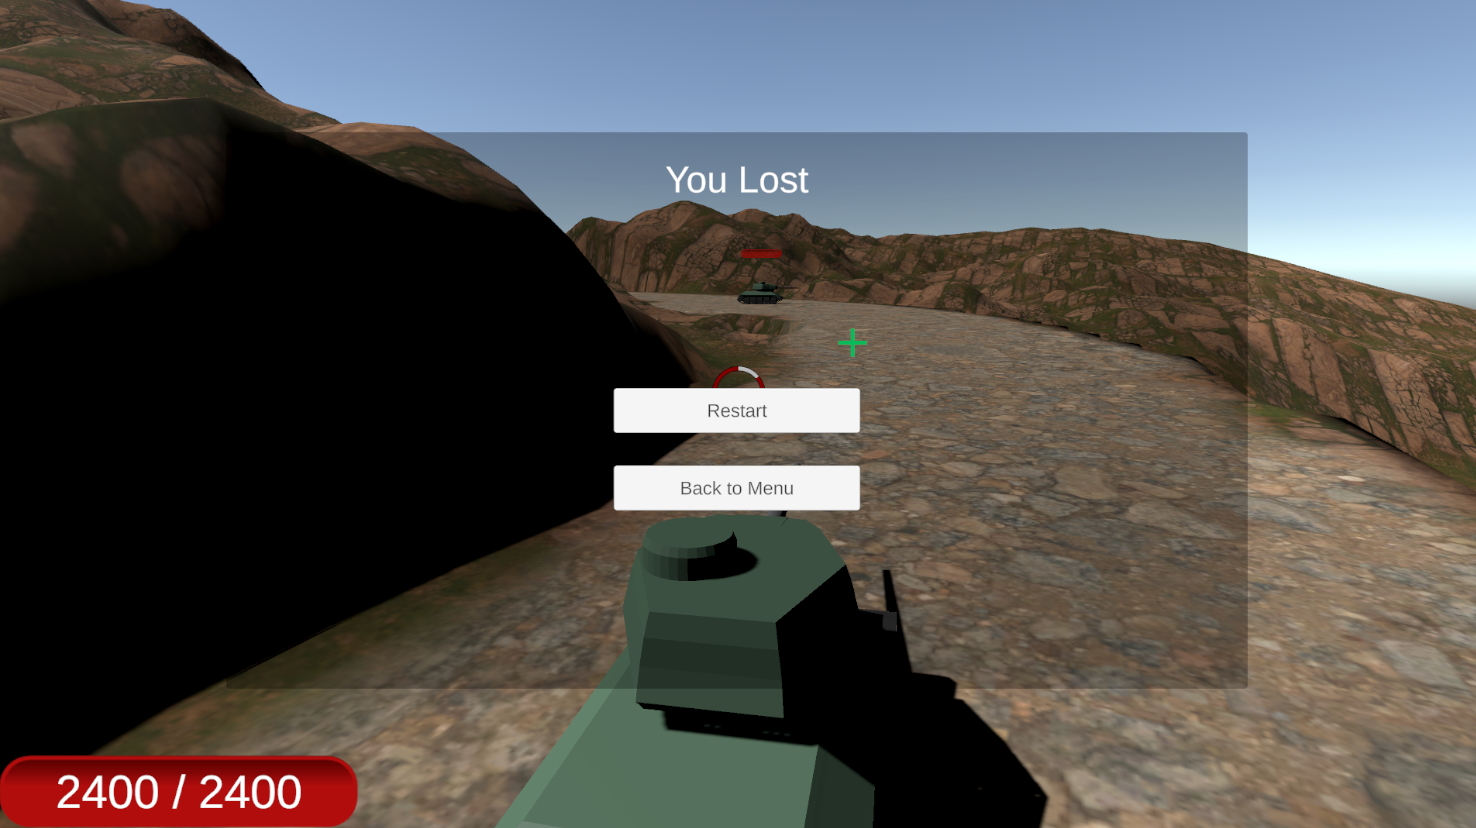
\includegraphics[width=0.9\textwidth]{screenshots/losegame.png}
    \caption{Az ellenség elérte az utolsó célpontot}
    \label{fig:losegame}
\end{figure}

A fejlesztői oldalon a tesztelés kicsit másképp történt, mivel itt a Unity-ba beépített \emph{Debug} osztály segítségével sokkal több információ volt elérhető. A leggyakrabban az osztály \emph{Log} metódusát használtam, melyet az értékek ellenőrzéséhez és események aktiválódásának jelzéséhez alkamaztam, például ha átment támadási módba az ellenség akkor az a Unity konzolában tisztán láttam. Emellett a \emph{Ray cast}-ek megjelenítésére a \emph{DrawRay} metódus nyújtott segítséget az ágyú jelenlegi irányának jelzésére, valamint ezt alkalmaztam még a játékos és az ellenség közötti irány megjelenítésére is.

\begin{figure}[H]
    \centering
    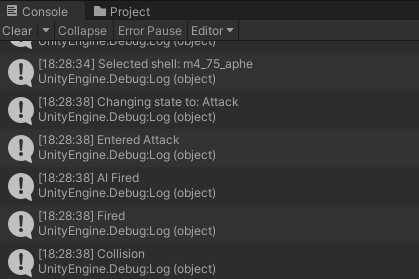
\includegraphics[width=0.7\textwidth]{screenshots/logging.png}
    \caption{Az események kiíratása a konzolba}
    \label{fig:logging}
\end{figure}

Több hiba is felbukkant a tesztelés során, mint például az ellenségek szokatlan viselkedése a támadási állapotban. Ebben az esetben a játékos lekövetése helyett inkább csak egy helyben állt és visszaváltott a járőrözési állapotba, később kiderült, hogy a kódban a problémát egy megfordított relációs jel okozta, ezt a hibát miután észleltem, sikeresen kijavítottam.

A tesztelés nagy segítséget nyújtott pár konstans érték finomítására is, mint például a fentebbiekben említett \emph{sidewaysFrictionFactor} beállításában, a lőszerek sebzésére, az ágyúk töltési hangolására, valamint kiegyensúlyozására is lehetőséget biztosított.

A tesztelésnek köszönhetően több hibát sikerült kijavítanom, és a játék megfelelő működését is megoldottam. A tesztelésben részt vevők egy új élményben részesültek, hozzájárultak a fejlesztés előrehaladásához és az élmény javításához is.

\chapter*{Összegzés}
\addcontentsline{toc}{chapter}{Összegzés}

Szakdolgozatom célja egy olyan új harckocsis játék megvalósítása volt, amihez hasonlóval korábban már játszottam, azonban miután néhány dolgot hiányoltam belőle, ezért úgy gondoltam, hogy az általam elképzelt játékot az én elképzeléseimnek megfelelően hozom létre, ezért számomra ennek a játéknak a kifejlesztése rengeteg kihívással járt.

Úgy érzem, hogy a projektnek az alapját és fő funkcióit sikerült az elvárásaimnak megfelelően kifejlesztenem. A lövedékekre és a páncélrendszer kifelszestésére kiemelt figyelmet fordítottam, így azt tartom a játék egyik fénypontjának.

Korábban Unity-vel és 3D modellezéssel még nem foglalkoztam igazán, ezért a játék kifejlesztése és a szakdolgozatom készítése során számtalan új tapasztalatot szereztem, melynek remélhetőleg hasznát tudom venni a jövőben.

A játék fejlesztése során többször elakadtam a tapasztalatom hiánya miatt, ezek áthidalása olykor kihívásnak bizonyult számomra, ami a játék pár részén meg is mutatkozik, ezért a jövőben szeretném ezeket finomítani és javítani. A 3D modelleket is szeretném jobb textúrákkal és több részlettel ellátni, hogy a napjainkban kiadott játékok szintjét elérje mind grafikában, mind élményben.

A projektem jelenlegi állapota készen áll több tartalom fogadására is, mely alatt főleg nagyobb harckocsi alkatrésztár és újabb pályák létrehozásását értem. Ezeket viszonylag egyszerűen lehetne hozzáadni, és újabb taktikákat tenne lehetővé.

A játék fejlesztése közben több ötletem is támadt újabb funkciók létrehozására, amikkel a jövőben szeretném a játékot kiegészíteni. Amit a legfontosabbnak tartok, az a kontrolleres bevitel támogatása és a billentyűk megváltoztatásának lehetősége az egyéni testreszabhatóság érdekében. Ezen kívül terveim között szerepel többféle ellenfél-viselkedést és játékmódot implementálni, valamint animációkat és esetlegesen vizuális fizikát hozzáadni a lánctalpakhoz.

Összességben a szakdolgozatom során sikerült megvalósítanom a tervezett funkciókat és rengeteg tapsztalatot szerezenem, valamint egy bepillantást kaptam a játékfejleszés világba is.


\begin{thebibliography}{55}

    \bibitem{warthunder}
    \textsc{Wikipedia} \emph{War Thunder} \\
    \url{https://en.wikipedia.org/wiki/War_Thunder} Megtekintés dátuma: 2025.04.14.

    \bibitem{navmesh}
    \textsc{Wikipedia} \emph{Navigation mesh} \\
    \url{https://en.wikipedia.org/wiki/Navigation_mesh} Megtekintés dátuma: 2025.03.29.

    \bibitem{raycast}
    \textsc{Wikipedia} \emph{Ray casting} \\
    \url{https://en.wikipedia.org/wiki/Ray_casting} Megtekintés dátuma: 2025.0.30.

    \bibitem{unity}
    \textsc{Wikipedia} \emph{Unity (Game Engine)} \\
    \url{https://en.wikipedia.org/wiki/Unity_(game_engine)} Megtekintés dátuma: 2025.03.31.

    \bibitem{GameObject}
    \textsc{Unity Documentation} \emph{GameObject} \\
    \url{https://docs.unity3d.com/Manual/class-GameObject.html} Megtekintés dátuma: 2025.04.03.

    \bibitem{components}
    \textsc{Unity Documentation} \emph{Components} \\
    \url{https://docs.unity3d.com/Manual/Components.html} Megtekintés dátuma: 2025.04.03.

    \bibitem{monobehavior}
    \textsc{Unity Documentation} \emph{MonoBehaviour} \\
    \url{https://docs.unity3d.com/Manual/class-MonoBehaviour.html} Megtekintés dátuma: 2025.04.03.

    \bibitem{transform}
    \textsc{Unity Documentation} \emph{Transform} \\
    \url{https://docs.unity3d.com/Manual/scripting-transform.html} Megtekintés dátuma: 2025.04.03.

    \bibitem{meshrenderer}
    \textsc{Unity Documentation} \emph{Mesh Renderer component reference} \\
    \url{https://docs.unity3d.com/Manual/class-MeshRenderer.html} Megtekintés dátuma: 2025.04.03.

    \bibitem{collider}
    \textsc{Unity Documentation} \emph{Collision} \\
    \url{https://docs.unity3d.com/Manual/collision-section.html} Megtekintés dátuma: 2025.04.03.

    \bibitem{rigidbody}
    \textsc{Unity Documentation} \emph{Rigidbody physics} \\
    \url{https://docs.unity3d.com/Manual/rigidbody-physics-section.html} Megtekintés dátuma: 2025.04.03.

    \bibitem{scripting}
    \textsc{Unity Documentation} \emph{Scripting} \\
    \url{https://docs.unity3d.com/Manual/scripting.html} Megtekintés dátuma: 2025.04.04.

    \bibitem{start}
    \textsc{Unity Documentation} \emph{MonoBehaviour.Start()} \\
    \url{https://docs.unity3d.com/ScriptReference/MonoBehaviour.Start.html} Megtekintés dátuma: 2025.04.04.

    \bibitem{update}
    \textsc{Unity Documentation} \emph{MonoBehaviour.Update()} \\
    \url{https://docs.unity3d.com/ScriptReference/MonoBehaviour.Update.html} Megtekintés dátuma: 2025.04.04.

    \bibitem{fixedupdate}
    \textsc{Unity Documentation} \emph{MonoBehaviour.FixedUpdate()} \\
    \url{https://docs.unity3d.com/ScriptReference/MonoBehaviour.FixedUpdate.html} Megtekintés dátuma: 2025.04.04.

    \bibitem{oncollisionenter}
    \textsc{Unity Documentation} \emph{Collider.OnCollisionEnter(Collision)} \\
    \url{https://docs.unity3d.com/ScriptReference/Collider.OnCollisionEnter.html} Megtekintés dátuma: 2025.04.04.

    \bibitem{ontriggerenter}
    \textsc{Unity Documentation} \emph{Collider.OnTriggerEnter(Collider)} \\
    \url{https://docs.unity3d.com/ScriptReference/Collider.OnTriggerEnter.html} Megtekintés dátuma: 2025.04.04.

    \bibitem{armoridea}
    \textsc{Github} \emph{ekmekodlamayoutube\_eng} \\
    \url{https://github.com/ekmekarasikodlama/ekmekodlamayoutube_eng} Megtekintés dátuma: 2025.04.07.

    \bibitem{rotation}
    \textsc{Unity Forums} \emph{Rotate towards target position (mouse) at a limited speed} \\
    \url{https://discussions.unity.com/t/rotating-slowly-toward-a-target-while-also-moving-toward-that-target/886726} Megtekintés dátuma: 2025.04.07.

    \bibitem{selectionmenu}
    \textsc{Youtube} \emph{Unity Character/Skin Selection Menu} \\
    \url{https://www.youtube.com/watch?v=2PKBChN10us} Megtekintés dátuma: 2025.04.07.

    \bibitem{inputsystem}
    \textsc{Youtube} \emph{How to use Unity's New INPUT System EASILY} \\
    \url{https://www.youtube.com/watch?v=HmXU4dZbaMw} Megtekintés dátuma: 2025.04.07.

    \bibitem{pitagorasz}
    \textsc{Wikipedia} \emph{Pitagorasz tétel} \\
    \url{https://hu.wikipedia.org/wiki/Pitagorasz-t\%C3\%A9tel} Megtekintés dátuma: 2025.04.08.

    \bibitem{demarre}
    \textsc{The Tank Archives} \emph{Penetration Equations} \\
    \url{https://www.tankarchives.ca/2014/10/penetration-equations.html} Megtekintés dátuma: 2025.04.08.

    \bibitem{freesound}
    \textsc{Freesound} \emph{Freesound} \\
    \url{https://freesound.org/} Megtekintés dátuma: 2025.04.08

    \bibitem{polyhaven}
    \textsc{Poly Haven} \emph{The Public 3D Asset Library} \\
    \url{https://polyhaven.com/} Megtekintés dátuma: 2025.04.10

    \bibitem{manualtesting}
    \textsc{Wikipedia} \emph{Manual testing} \\
    \url{https://en.wikipedia.org/wiki/Manual_testing} Megtekintés dátuma: 2025.04.12

\end{thebibliography}
\addcontentsline{toc}{chapter}{\bibname}


\includepdf{nyilatkozat.pdf}

\end{document}
